%%
%% This is file `sample-authordraft.tex',
%% generated with the docstrip utility.
%%
%% The original source files were:
%%
%% samples.dtx  (with options: `authordraft')
%% 
%% IMPORTANT NOTICE:
%% 
%% For the copyright see the source file.
%% 
%% Any modified versions of this file must be renamed
%% with new filenames distinct from sample-authordraft.tex.
%% 
%% For distribution of the original source see the terms
%% for copying and modification in the file samples.dtx.
%% 
%% This generated file may be distributed as long as the
%% original source files, as listed above, are part of the
%% same distribution. (The sources need not necessarily be
%% in the same archive or directory.)
%%
%% The first command in your LaTeX source must be the \documentclass command.

\documentclass[sigconf]{acmart}
\usepackage{multirow}
\usepackage{xspace}
\usepackage{spreadtab}
\usepackage[inline]{aplcomments}
\newcommenter{shan}{1.0,0.0,0.0}
\newcommenter{junwen}{0.0,1.0,0.0}
\newcommenter{cong}{0.0,0.8,0.8}
\newcommenter{alvin}{0.0,1.0,1.0}
\usepackage{listings}
\lstloadlanguages{Ruby}
\lstset{%
basicstyle=\ttfamily\color{black},
commentstyle = \ttfamily\color{blue},
keywordstyle=\ttfamily\color{blue},
stringstyle=\color{orange}}
\lstset{emph={User, @comment, comments, user, Comment},emphstyle={\color{red}}
}

\newcommand{\Tool}{EvolutionSaver\xspace}
\newcommand{\numRailsApp}{6\xspace}
\newcommand{\numDjangoApp}{6\xspace}
\newcommand{\numRailsError}{73\xspace}
\newcommand{\numRailsWarning}{25\xspace}
\newcommand{\numDjangoError}{xx\xspace}
\newcommand{\numDjangoWarning}{xx\xspace}
%% NOTE that a single column version may be required for 
%% submission and peer review. This can be done by changing
%% the \doucmentclass[...]{acmart} in this template to 
%% \documentclass[manuscript,screen,review]{acmart}
%% 
%% To ensure 100% compatibility, please check the white list of
%% approved LaTeX packages to be used with the Master Article Template at
%% https://www.acm.org/publications/taps/whitelist-of-latex-packages 
%% before creating your document. The white list page provides 
%% information on how to submit additional LaTeX packages for 
%% review and adoption.
%% Fonts used in the template cannot be substituted; margin 
%% adjustments are not allowed.
%%
%% \BibTeX command to typeset BibTeX logo in the docs
% \AtBeginDocument{%
%   \providecommand\BibTeX{{%
%     \normalfont B\kern-0.5em{\scshape i\kern-0.25em b}\kern-0.8em\TeX}}}

%% Rights management information.  This information is sent to you
%% when you complete the rights form.  These commands have SAMPLE
%% values in them; it is your responsibility as an author to replace
%% the commands and values with those provided to you when you
%% complete the rights form.
% \setcopyright{plain}
% \copyrightyear{2018}
% \acmYear{2018}
% \acmDOI{10.1145/1122445.1122456}

% %% These commands are for a PROCEEDINGS abstract or paper.
% \acmConference[Woodstock '18]{Woodstock '18: ACM Symposium on Neural
%   Gaze Detection}{June 03--05, 2018}{Woodstock, NY}
% \acmBooktitle{Woodstock '18: ACM Symposium on Neural Gaze Detection,
%   June 03--05, 2018, Woodstock, NY}
% \acmPrice{15.00}
% \acmISBN{978-1-4503-XXXX-X/18/06}


%%
%% Submission ID.
%% Use this when submitting an article to a sponsored event. You'll
%% receive a unique submission ID from the organizers
%% of the event, and this ID should be used as the parameter to this command.
%%\acmSubmissionID{123-A56-BU3}

%%
%% The majority of ACM publications use numbered citations and
%% references.  The command \citestyle{authoryear} switches to the
%% "author year" style.
%%
%% If you are preparing content for an event
%% sponsored by ACM SIGGRAPH, you must use the "author year" style of
%% citations and references.
%% Uncommenting
%% the next command will enable that style.
%%\citestyle{acmauthoryear}

%%
%% end of the preamble, start of the body of the document source.
\begin{document}

%%
%% The "title" command has an optional parameter,
%% allowing the author to define a "short title" to be used in page headers.
\title{Automatic Refactoring for  Database-Backed Web Applications based on Schema Changes}

%%
%% The "author" command and its associated commands are used to define
%% the authors and their affiliations.
%% Of note is the shared affiliation of the first two authors, and the
%% "authornote" and "authornotemark" commands
%% used to denote shared contribution to the research.
\author{Sophie Xie}
\email{sxie2@cps.edu}
\affiliation{%
  \institution{Whitney Young High School}
  \country{}
}
\author{Junwen Yang}
\email{junwen@uchicago.edu}
\affiliation{%
  \institution{University of Chicago}
  \country{}
}

\author{Shan Lu}
\email{shanlu@uchicago.edu}
\affiliation{%
  \institution{University of Chicago}
  \country{}
}

%%
%% By default, the full list of authors will be used in the page
%% headers. Often, this list is too long, and will overlap
%% other information printed in the page headers. This command allows
%% the author to define a more concise list
%% of authors' names for this purpose.


%%
%% The abstract is a short summary of the work to be presented in the
%% article.
\begin{abstract}
Modern web applications manipulate a large amount of user data and undergo frequent data-schema changes. These changes bring up a unique refactoring 
task: updating application code to be consistent with data schema. Previous
 study and our own investigation show that this type of refactoring is 
error-prone and time-consuming for developers.
%Schema change requires drastic change in application's implementation.  It's error-prone and non-trivial to keep the application code consistent with the schema change, especially when web applications are often constructed using Object-Relational Mapping frameworks, which allows developers to manipulate persistent data using object-oriented code. Tool support is needed to fulfill this task. 
This paper presents \Tool, a static code analysis and transformation tool that
automates schema-related code refactoring and consistency checking. 
\Tool is implemented as an IDE 
plugin that works for both Rails and Django applications. 
%\Tool extracts the schema change, and detects application code which is affected by the schema change and applies fixes automatically. 
The source code of \Tool is available on Github~\cite{sourcecode} and the plugin can be downloaded from Visual Studio Marketplace~\cite{vscodemarketplace}, with its tutorial available at \url{https://www.youtube.com/watch?v=qBiMkLFIjbE}. 
\end{abstract}

%%
%% The code below is generated by the tool at http://dl.acm.org/ccs.cfm.
%% Please copy and paste the code instead of the example below.
%%
% \begin{CCSXML}
% <ccs2012>
%  <concept>
%   <concept_id>10010520.10010553.10010562</concept_id>
%   <concept_desc>Computer systems organization~Embedded systems</concept_desc>
%   <concept_significance>500</concept_significance>
%  </concept>
%  <concept>
%   <concept_id>10010520.10010575.10010755</concept_id>
%   <concept_desc>Computer systems organization~Redundancy</concept_desc>
%   <concept_significance>300</concept_significance>
%  </concept>
%  <concept>
%   <concept_id>10010520.10010553.10010554</concept_id>
%   <concept_desc>Computer systems organization~Robotics</concept_desc>
%   <concept_significance>100</concept_significance>
%  </concept>
%  <concept>
%   <concept_id>10003033.10003083.10003095</concept_id>
%   <concept_desc>Networks~Network reliability</concept_desc>
%   <concept_significance>100</concept_significance>
%  </concept>
% </ccs2012>
% \end{CCSXML}

% \ccsdesc[500]{Computer systems organization~Embedded systems}
% \ccsdesc[300]{Computer systems organization~Redundancy}
% \ccsdesc{Computer systems organization~Robotics}
% \ccsdesc[100]{Networks~Network reliability}

%%
%% Keywords. The author(s) should pick words that accurately describe
%% the work being presented. Separate the keywords with commas.
% \keywords{datasets, neural networks, gaze detection, text tagging}

%% A "teaser" image appears between the author and affiliation
%% information and the body of the document, and typically spans the
%% page.
% \begin{teaserfigure}
%   \includegraphics[width=\textwidth]{sampleteaser}
%   \caption{Seattle Mariners at Spring Training, 2010.}
%   \Description{Enjoying the baseball game from the third-base
%   seats. Ichiro Suzuki preparing to bat.}
%   \label{fig:teaser}
% \end{teaserfigure}

%%
%% This command processes the author and affiliation and title
%% information and builds the first part of the formatted document.
\renewcommand\footnotetextcopyrightpermission[1]{}
\settopmatter{printacmref=false} 
\pagestyle{plain}

\maketitle

\section{Introduction}
\label{sec:intro}
Modern web applications often use database engines to 
manage a large amount of user data, such as user profiles in social network applications and transaction
records in on-line shopping platforms~\cite{webapp}.  
The schema of such data goes through changes, such as table renaming, column
deletion, and others, for better performance or functionality when an application evolves \cite{wang2017verifying}.
Unfortunately, it is difficult for developers to keep their code 
consistent with database schema changes all the time, a task we
refer to as \textit{schema-related code refactoring}, with any inconsistency leading
to application crashes.

Schema-related refactoring and
traditional refactoring like class renaming share similarities, given that
popular Object Relational Mapping (ORM) frameworks, such as Rails \cite{rails},  
Django \cite{django}, and Hibernate \cite{hibernate},
allow database data to be
updated and retrieved in an object-oriented way---the name of a database table corresponds to the name of a model class
and the names of table columns are the same as class fields.

%\shan{TODO: we may need to expand the onebody example}
However, they also differ in various aspects, due to the unique nature of persistent data,
as we elaborate below\footnote{Our discussion generally applies to
all web applications developed upon ORM frameworks, although our
examples use Ruby on Rails applications.}.



%Comparing with traditional software, database-backed web applications face the unique code-maintenance challenge of making code changes consistent with database schema changes. Because web applications are often constructed using Object Relational Mapping (ORM) frameworks allowing the properties and relationships of the objects in an application to be easily stored and retrieved from a database in an object-oriented way, which can go beyond the form of class name and field name as used in traditional software, e.g.,  in line 2 in listing~\ref{onebody-query}, the \texttt{sequence} column of \texttt{people} table is used as a parameter of \texttt{order} function call in the form of string. 



% The class definition in database-backed web applications  will not explicitly declare its fields since database columns  will be mapped to the fields by ORM frameworks implicitly. 
% ORM frameworks will implicitly map database columns to the object's class. 
 


% \begin{lstlisting}[float=t,language=Ruby,label={onebody-query}, caption=Inconsistent code from Onebody]
% app/controllers/checkin/families_controller.rb
%     # select * from people where family_id = ? 
%     # and is_deleted = ? order by sequence
% 1   @family.people.undeleted.order('sequence')

% app/models/person.rb
% 2   person.sequence = 1
% \end{lstlisting}
% For example, in Spree \cite{spree}, an online-shopping application, a table named orders is used to 
% keep the order information. In one version, 
% developers renamed a column in this table from \texttt{guest\_token} to \texttt{token} since the column starts to store \texttt{tokens} used in login cookies for not only guest but also general users\shan{what does token mean? what does general token mean?}, it has to change all the references to the old name \texttt{guest\_token} to the new name \texttt{token}, which results in 284 lines of code change across 32 files. 
%It's challenging for developers to manually refactor the application code based on the schema change. 

\textit{How is schema defined?} Different from a regular class whose 
field names and field types are defined by its class
declaration, a model class's structure has to match its corresponding database table that is created once at an application's installation or upgrade.
%with its data retrieved into objects at run time.
In fact, in some ORM frameworks like Rails, persistent fields of a model class are \textit{not} declared in its class
definition and are instead automatically mapped by Rails from the corresponding table schema, which is 
%Consequently, although every table (e.g., \texttt{people}) corresponds to a class
%with a singularized name (e.g., \texttt{Person}), the schema, including table names, column
%names and types, and other information, has to be 
defined through ORM
APIs like \texttt{create\_table} in Rails or
\texttt{CreateModel} in Django in a type of files called
\textit{migration files},
as shown in Listing \ref{migration}. 
%In fact, the corresponding model class definition needs not contain definitions of column fields.

\textit{How is schema changed?} 
%One cannot change the
%schema (e.g., a column name) by changing the class definition. 
Schema changes are expressed
through ORM APIs in migration files (e.g., line 4 in Listing 
\ref{migration}
renames the column \texttt{sequence} in table \texttt{people}), 
which informs the web application about how to 
update its database during installation and upgrade.
In an ORM framework like Rails, schema changes cannot be seen in
class definitions.

\lstinputlisting[float=t, basicstyle=\footnotesize\ttfamily, label={migration}, caption={Migration files from Onebody},language=Ruby]{migration.rb}

\lstinputlisting[float=t,basicstyle=\footnotesize\ttfamily, label={onebody-query}, caption={Inconsistent code from Onebody},language=Ruby]{onebody-query.rb}

\textit{What code refactoring is needed?} Following a schema
change in the migration file, corresponding references in the
application need to change. Some of these are just
class or field renaming like in line 2 of Listing \ref{onebody-query}, while some require changing ORM APIs' parameters like in line 1 of Listing \ref{onebody-query}.
%and hence requires ORM knowledge.

For example, developers of Onebody~\cite{onebody}, a popular social network application, used 
a table \texttt{people} to keep user information. In one commit, they renamed the \texttt{sequence} column in \texttt{people} to \texttt{position} (line 4 in Listing \ref{migration}). In the same commit, they
correctly updated the reference to \texttt{sequence} in 6 places across 4 files like the one in line 2 of Listing \ref{onebody-query}, but forgot to change the other 5 places, 
such as the parameter reference shown in line 1 of Listing
\ref{onebody-query}. This inconsistency caused web users to
suffer from webpage crashes~\cite{onebodyissue672}.
%\url{https://github.com/seven1m/onebody/issues/672}}
%\shan{the issue report does not read like application crash.}

%https://github.com/spree/spree/pull/8826/files

% Moreover, the challenge is escalated by the prevalent usage of Object-Relational Mapping (ORM) frameworks, such as Ruby on Rails~\cite{rails}, Django for Python~\cite{django}, and Hibernate for Java~\cite{django}. Because they provide a convenient way for developers to evolve their database schema over time using object-oriented code without issuing `ALTER TABLE' SQL commands to database, which eases the efforts and results in more frequent schema change. 
% \shan{Do you have evidence that there are more frequent schema changes in ORM applications?
% If not, I don't think we can claim it. I can imagine maybe it is more error prone, because
% schema changes and declaration are in different files from files that use the tables and columns,
% so that it is more isolated ... I don't know ...} 
% \junwen{I have found that in an empirical study on web application not using ORM framework~\cite{qiu2013empirical}, the average schema change per release is 60, so we cannot draw the conclusion that orm schema changes faster. But their way of calculating change is to check every revision instead of every release. We may change our counting methodology and regenerate the result. 
% }


%TODO:\shan{There needs to be a clearer definition of what are code-schema inconsistencies.}
%TODO:\shan{can some of the inconsistency get exposed by unit testing? }
% Inconsistency between application code and its data schema could cause web-page crashes 
% with database exceptions thrown 
% Different from traditional software, the object class's fields in database-backed web applications are not declared explicitly in the class itself but mapped to the database columns by ORM frameworks implicitly
 
% Thus, existing refactoring tools that tackle method or field renaming are not able to refactor the database-backed web applications.

Recent work motivated tool support for schema-related refactoring  \cite{wang2017verifying} and proposed techniques to synthesize updates to a list of 
SQL queries given the old schema and the new schema written in SQL
\cite{wang2019synthesizing}. Although inspiring, it does not directly help
many web applications, whose schema changes
and database operations are expressed in ORM APIs, rarely if ever in raw SQL.

%As a result, cross-stack analysis which combines the database information with application code is necessary to detect and fix the inconsistency  between application code and schema change. 
%Existing work MIGRATOR~\cite{wang2019synthesizing} can automatically synthesize database program after schema refactor, however it can only work on database programs written in SQL. 
% Also, MIGRATOR is guessing value correspondence from the name of table and column of two schema\shan{I don't understand}, which is possible to cause inaccurate mapping and generate incorrect refactoring. Also, MIGRATOR is not able to handle deletion change. \shan{I don't understand.} 



This paper presents {}, a tool that uses ORM-aware static analysis to help schema-related code refactoring in web applications
written in Rails \cite{rails} and Django \cite{django}, two popular web frameworks.
%\shan{can we say 'most' popular? can we say web application frameworks, instead of ORM frameworks to make it sound more general?}. \junwen{According to the data \url{https://www.statista.com/statistics/1124699/worldwide-developer-survey-most-used-frameworks-web/}, Django and Rails are not the most popular web app frameworks. But based on data we collected on github before, for apps with more than 100 starts, the most popular is Rails and then django}
Given two versions of a web application, 
\ETool{} analyzes and identifies schema changes from
migration files, searches for
any code inconsistent with the new schema,
and generates warnings and patches accordingly. %\shan{Why do we need the old code version? If I just give you one version,can you identify code--schema inconsistency?} \junwen{Yes, we can. Having the old version schema is to just make the detection even faster by only checking on the changed schema}.

%As an IDE plugin, \ETool{} supports two usage scenarios: 1) it can semi-automate \shan{why semi? what is not automated?} the refactoring for an old application after users make data-schema changes \shan{what type of data schema changes do you support? What is the scope/limitations of your tool?}. 2) it can identify remaining inconsistency between the data schema and the application code, after
%developers commit changes to both data schema and the application code.  %\shan{I can imagine two potential uses of this type of tools: (1) once a data schema change is made, it will help automate or semi-automate all the needed code changes; (2) given a data schema change AND changed software, it checks if there are inconsistency between the data schema and the software. Does your tool only offer functionality-2? Or do you offer both? I guess you offer both, if so, you should rephrase the usage flow and functionality description of your tool.} 
%This work makes the following contributions:


%\shan{What type of guarantees you can offer here? Do you guarantee that you will generate perfectly correct and complete refactoring?} 

To ease its adoption, we have integrated \ETool into the popular 
Visual Studio Code IDE~\cite{vscodepop} as a plugin. Web developers can use this plugin to
guide their schema-related refactoring or to look for
schema--code inconsistency bugs.

In our evaluation with 12 popular Rails and Django applications, 
\ETool detected \numRailsError schema--code inconsistencies 
%in 72 files 
caused by 35 schema changes in the past.
%and 25 warnings caused by 4 schema changes in application code that are caused by schema changes.  Among the 80 errors, 
We have reported 11 of them that exist in the latest versions to developers,
and got 10 of them already confirmed and 6 of them already patched based on
our suggestion.
Our examination of the rest \numFixed inconsistencies shows that 
they took many days for developers
to discover and fix.
%they took 378 days and 3 days on average for Rails and Django developers to discover and fix, respectively. %Moreover, \numfixedafterrelease of them are fixed after the version release. 

\ETool's source code is on Github~\cite{sourcecode} and the plugin can be downloaded from Visual Studio Marketplace~\cite{vscodemarketplace}.


\section{Schema Changes}
% Please add the following required packages to your document preamble:
% \usepackage{multirow}
%\label{change}


%Schema changes include addition, deletion, renaming on table, column, association, index, and constraint, and type change on association and column. For example, a column could change from a `int' type to a `string' type. And an association could change from `has\_one' to `has\_many'.  

\textbf{Extended motivation.}
A recent study~\cite{wang2017verifying} on 100 Rails applications 
%with more than 400 commits 
showed that most applications went through many schema changes.
%are common: about 28 per application on average.
%database schema has been changed at least once in all these 100 applications, with the average 
%about 28 schema changes on average over each application's life time.  
For further motivation, we studied
12 Rails and Django web applications from different categories like forum, e-commerce, social network, etc. \footnote{The application list is in our code
repository.} They are all highly rated, each with
more than 1000 stars on GitHub, 11,000--900,000 lines of code and 500--100,000 commits. 


% Schema change could happen on table, columns, associations, and indices
% % \junwen{Isil's group also shows constraints change, we didn't since it's covered in previous paper and will not cause query issue}; 
% a change could be addition, deletion, renaming. Besides, for column and association, it also contains type change. For example, a column could change from a `int' type to a `string' type. And an association could change from `has\_one' to `has\_many'. 
% \begin{table}[]
\caption{Application Corpus}
\label{tab:apps}
\resizebox{1\columnwidth}{!}{
\begin{tabular}{llrrrr}
\hline
\hline
Name & Category & \# stars & \# commits & \# versions & \# loc \\
\hline
Lobsters & Forum & 3k & 2.1k & 19 & 11 k \\
Gitlab & Collaboration & 22.6k & 100k & 1040 & 932k \\
Spree & E-commerce & 11.3k & 23.4k & 244 & 74k \\
Tracks & Management & 1k & 4.4k & 19 & 16k \\
Diaspora & Social Network & 12.7k & 20k & 82 & 83k \\
Onebody & Social Network & 1.4k & 5.2k & 32 & 103k \\
\hline
Zulip &  Collaboration & 13.7k  & 42.5k & 78 & 162k \\
Awx & Management & 9.7k & 29.7k & 45 & 93k \\
Saleor & E-commerce & 11.1k & 18.5k & 142 & 174k \\
Healthchecks & Management & 3.8k & 1.7k & 26 & 17k \\
Gerapy & Management  & 2.4k & 0.5k & 26 & 22k \\
Posthog &  Collaboration & 4.1k & 3.1k & 52 & 39k \\
\hline
\hline
\end{tabular}
}
\end{table}

\textit{How often are schema changes?} 18\% -- 85\% of application versions
contain at least one schema change, and there are more than 8 changes for every
version on average.
Furthermore, changes are common throughout the development history of each
application. For example, across the 6 Rails applications, the most recent 25\%
of commits happen to contain about 25\% of all the schema
changes in total.

%, as shown in Table~\ref{tab:change-stat}.
%Note that, for all  applications except for Lobsters \cite{lobsters}, we treat every public code release as a version; since Lobsters does not specify code release/version, we treat every 100 code commits as one version. 

\textit{What types of changes are there?} As shown in Table \ref{tab:change-stat},
 changes to various aspects of the schema
 %tables, columns, association relationships (e.g., `has\_one'
%or `has\_many' relationship between two tables), and table indices, 
are all common.
About three quarters of changes add tables, columns, or indices, and
do not directly cause inconsistency with existing code. The remaining
one quarter of changes modify or delete existing tables, columns,
associations, or indices, immediately threatening code consistency, and hence
are the target of \ETool, as detailed
in Table \ref{tab:overview}.


\iffalse 
\textbf{How schema changes vary with age?} We split every application' history into four quarters, each with the same number of releases/versions and count the average number of schema changes in each quarter (time gaps between code releases
are stable within each application). As shown in Figure~\ref{fig:evo-time}, although there are more changes in the first two quarters, changes in the latter two quarters
are still common.
%, indicating that schema-related refactoring is necessary for applications at any development stage no matter it's new or mature. 
%\shan{If you want to save space, you can replace Figure 1 with a text explanation saying how many changes are there in each major version: I assume there are 13 major versions for AWX? Based on AWX, I feel there are indeed more schema changes at the beginning, but there are still a good amount of changes lat j er on. That is probably a more fair claim.}


\begin{figure}
    \centering
    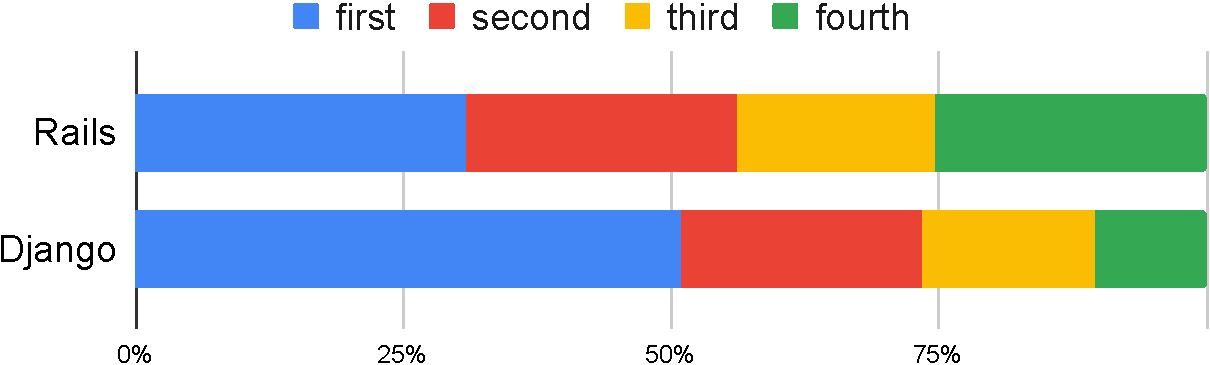
\includegraphics[width=\columnwidth]{figs/breakdown-4.pdf}
    \caption{Quarter Breakdown of Schema Changes (Aggregated View)}
    \label{fig:evo-time}
\end{figure}
% \shan{Explain how is your study different from that by
% Isil's group. It is also fine if your study is similar
% with Isil's group's study, and just that you look at different sets of applications. No matter what is the case, please explain clearly.}
\fi 


% \shan{need to introduce these applications a bit. why you choose these applications to study; how large they are; how long they have been under development, etc.}

%Overall, schema changes of various types broadly exist in applications across their development phases. Related refactoring support will be broadly beneficial.






\begin{table}
\caption{Number of Schema Changes per Version}
\label{tab:change-stat}
\centering
%\setlength{\tabcolsep}{2pt} 
%\resizebox{\columnwidth}{!}{
\begin{tabular}{lrrrrr}
\arrayrulecolor{black}\hline  
\arrayrulecolor{black}\hline
Change Target  & Table  & Column  & Association  & Index  & Total \\
\arrayrulecolor{black}\hline
Django & 1.0           & 4.4            & 2.6                & 0.2     & 8.2      \\
Rails  & 1.6           & 4.8            & 2.2                & 1.3  & 9.9     \\   
\arrayrulecolor{black}\hline  
\arrayrulecolor{black}\hline
\end{tabular}
% \begin{tabular}{l|rr}

% \arrayrulecolor{black}\hline  
% \arrayrulecolor{black}\hline
% Types & Django  &  Rails \\ \hline
% Table Changes & 1.1 & 1.6 \\
% Column Changes & 4.7 & 4.8 \\
% Association Change & 2.5 & 2.2 \\
% Index Changes & 0.1 & 1.3 \\ 
% \hline
% Total & 8.4 & 9.8 \\

% \arrayrulecolor{black}\hline  
% \arrayrulecolor{black}\hline
% \end{tabular}
%}
\end{table}






\section{Approach}
This section presents our approach to refactoring the application code based on schema change in four steps, which are schema change extraction, query extraction, inconsistency detection, and patch generation \shan{``solution generation'' sounds strange}. Some code snippets will be utilized as examples which are mainly from Rails applications. But similar APIs and usage exist in Django applications as well. 

\label{sec:app}
%\subsection{Overview}
Figure~\ref{fig:app} shows the overview of our approach.
For each HTML element rendered on the webpage, we calculate the performance cost on it including the wall-clock real-time cost and relative cost towards the database size. This performance information will be displayed on the webpage after it's loaded inside the Browser. And then, for each HTML element, we provide the possible design opportunities. Once developers choose one design opportunity for certain HTML element, the source code will be edited to satisfy the developers' requirement.
\begin{figure}[H]
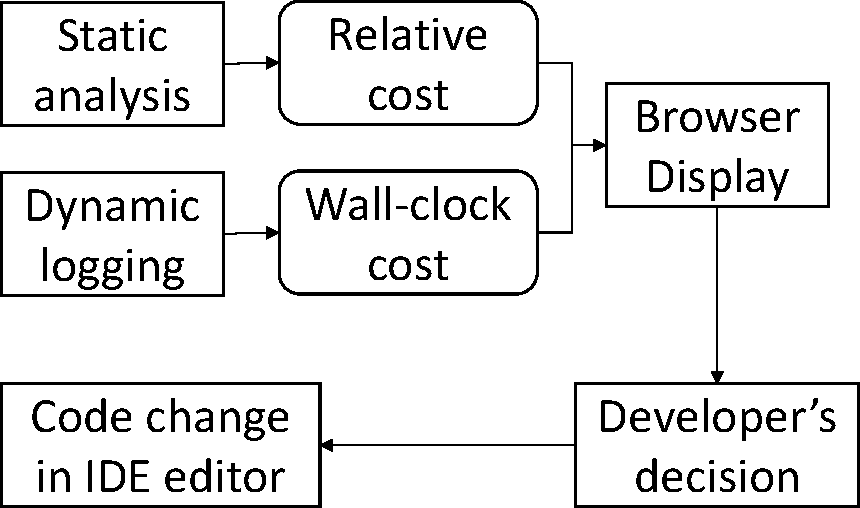
\includegraphics[width=\columnwidth]{figs/p2-crop.pdf}
\caption{Overview of Approach}
\label{fig:app}
\end{figure}
\subsection{Performance Cost Estimation}
We estimates the performance cost for each HTML tag that will be rendered on the page through dynamic run-time logging and static analysis, which is a new granularity for performance estimation. Also our approach includes the wall-clock performance cost and relative performance cost towards the database size. As a result, this approach also works when there is not a representative workload for us to gain enough performance cost information. 
 
\subsection{Interactive Design Interface}
We propose a brand new interface for web application design. We firstly render the performance cost information estimated from last step on the web page for each HTML tag. And for those HTML tags that take large performance cost, we identify the possible alternative design choices from these options: (1) pagination, (2) approximation, (3) asynchronous loading, and (4) removing. Developers are allowed to choose their desired design choice. After developers' selection, source code will be automatically revised so that the application can achieve their wanted behavior. The performance cost of updated application will re-estimated and displayed on the web page in order that the performance improvement can be observed. 





% \shan{I hope you will tell me what type of problems your tool look at (what type of issues your tool detect) here.} 

\section{\Tool{} IDE INTEGRATION}
\subsection{Features of \Tool{} IDE plugin}

\begin{figure*}
\centering
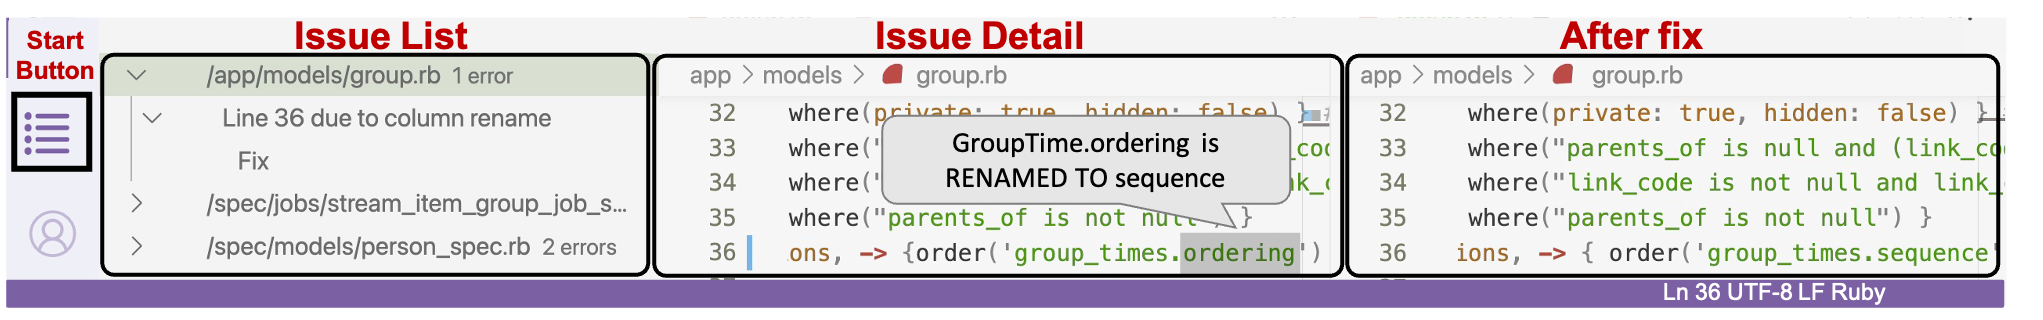
\includegraphics[width=\textwidth]{figs/plugin.png}
\caption{The screenshot of \Tool{} IDE Plugin}
\label{fig:vscode-plugin}
\end{figure*}


We have implemented \Tool{} as a plugin for Visual Studio Code~\cite{vscode}, a popular IDE for multiple languages.
% \shan{citation needed to back this claim up}
As shown in Figure~\ref{fig:vscode-plugin}, one can press the start button to start the plugin. By default, \Tool compares the current code with the latest commit.
% \shan{can I specify which commit to compare against? 
%If this is not difficult to implement, it would be nice to have}. 
Users can also specify the commits they desire to check in the configuration file. 

\textbf{Issue list.} The left panel, as shown in Figure~\ref{fig:vscode-plugin}, lists all the errors detected by \Tool in a hierarchical view. The first level lists
the files where errors are detected; clicking a file shows the details of every 
error in that file, including the line number and the type of root-cause schema change;
clicking the error shows a ``Fix'' button. 

\textbf{Issue detail.} Clicking a file in the issue list will navigate users to the corresponding file in the editor, with the error code highlighted. Users can hover their mouses over the highlighted code and see the detailed
explanation, like ``GroupTime.ordering is RENAMED TO sequence'' in Figure~\ref{fig:vscode-plugin}. 

\textbf{Issues fix.} One can click the  `\texttt{Fix}'  button  on the left panel
or a `\texttt{Fix all}' button to fix one or all the issues.


\subsection{Implementation}
The start button triggers our static analyzer to run on the given
code commits. The analyzer produces an \texttt{output.json} file that is parsed 
%by \texttt{getDepsInPackageJson} 
to create the issue list using  the Visual Studio Code Extension APIs \texttt{TreeDataProvider} and \texttt{TreeItem}. 
The \texttt{DocumentHighlightProvider} API is used to highlight the selected error code, given the filename and line number information in 
\texttt{output.json}. The \texttt{HoverProvider} API enables the tooltip of detailed reason to  display once hovering over the highlighted code.
To fix the error, \texttt{TextDocument}, \texttt{Range}, and  \texttt{ExtensionContext} APIs are used to insert, replace, and delete source code in the editor panel.





\section{Evaluation}

\label{sec:eva}
Our evaluation focuses on four research questions:
{\bf RQ1}: Can \Tool identify view-aware optimization opportunities from latest versions
    of popular web applications?
{\bf RQ2}: How much performance benefits can view-aware optimization provide?
{\bf RQ3}: Is the performance-functionality trade-off space exposed by \Tool worthwhile for developers to explore?
{\bf RQ4}: Does \Tool estimator estimate the per-tag data-processing cost accurately?
\begin{table}[t]											
\centering											
\caption{Opportunities detected by \Tool in 12 apps}												
\label{tab:oppo}										\centering
\resizebox{0.6\columnwidth}{!}{%
\begin{tabular}{@{}lrrrrrrrrrrrrr@{}}
\toprule
App	&	Ds	&	Lo	&	Gi	&	Re	&	Sp	&	Ro	&	Fu	&	Tr	&	Da	&	On	&	FF	&	OS	&	SUM	\\	\midrule
pagi.	&	1	&	6	&	1	&	10	&	2	&	20	&	5	&	9	&	1	&	6	&	3	&	3	&	69	\\	\midrule
approx.	&	1	&	1	&	0	&	7	&	0	&	5	&	1	&	3	&	0	&	23	&	0	&	0	&	43	\\	\midrule
removal	&	1	&	2	&	0	&	7	&	0	&	4	&	1	&	2	&	2	&	2	&	0	&	0	&	22	\\	\midrule
asynch	&	1	&	2	&	0	&	2	&	0	&	2	&	1	&	2	&	2	&	2	&	0	&	0	&	15	\\	\midrule
SUM	&	4	&	11	&	1	&	26	&	2	&	31	&	8	&	16	&	5	&	33	&	3	&	3	&	149	\\	
 \bottomrule
\end{tabular}

}	
\end{table}

\begin{table}[h]
\centering
\caption{Speed up of 15 view changes}
\label{tab:speedup}
\resizebox{\columnwidth}{!}{%
\begin{tabular}{@{}l|rrrrrr|rr|rrrr|rrr@{}}
\toprule
%  & \multicolumn{6}{|c|}{Pagination} & \multicolumn{4}{c|}{Approximation} & \multicolumn{3}{c|}{Content Removal} & \multicolumn{2}{c}{ Asynchronous} \\ \midrule
% ID & Ro1 & Tr1 & Fu1 & Re2 & On1 & Re1 & Re2 & On2 & Tr2 & On3 & Lo1 & Re3 & On4 & Lo2 & On5 \\ \midrule
% Server Time Speedup (X) & 19.4 & 13.5 & 6.8 & 4.7 & 2.1 & 1.8 & 2.1 & 1.4 & 1.2 & 1.3 & 33.0 & 1.4 & 1.1 & 37.8 & 1.1 \\ \midrule
% End-to-End Time Speedup (X) & 9.4 & 9.2 & 5.9 & 3.6 & 2.7 & 1.6 & 1.6 & 1.3 & 1.2 & 1.0 & 8.7 & 1.3 & 1.2 & 17.2 & 1.2 \\
&	\multicolumn{6}{|c|}{Pagination}	&	\multicolumn{2}{c|}{	Asynchronous}	&	\multicolumn{4}{c|}{Approximation}	&	\multicolumn{3}{c}{Content	Removal}	\\	\midrule																													
ID	&	Ro1	&	Tr1	&	Fu1	&	Re2	&	On1	&	Re1	&	Lo2	&	On5	&	Re2	&	On2	&	Tr2	&	On3	&	Lo1	&	Re3	&	On4					\\	\midrule				
Server Time Speedup (X)	&	19.4	&	13.5	&	6.8	&	4.7	&	2.1	&	1.8	&	37.8	&	1.1	&	2.1	&	1.4	&	1.2	&	1.3	&	33	&	1.4	&	1.1					\\	\midrule				
End-to-end Time Speedup (X)	&	9.4	&	9.2	&	5.9	&	3.6	&	2.7	&	1.6	&	17.2	&	1.2	&	1.6	&	1.3	&	1.2	&	1	&	8.7	&	1.3	&	1.2					\\					
\bottomrule
\end{tabular}
}
{Every case is denoted by $<$application-short-name$>$-ID}
\end{table}

\begin{table*}[th]
\centering
\caption{Database sizes and page load time of 12 user-study cases}
\label{tab:dbsize}	
\resizebox{1\columnwidth}{!}{%
%\begin{tabular}{@{}l|ggg|ggg|ggg|ggg@{}}
\begin{tabular}{@{}l|ccc|ccc|ccc|ccc@{}}
\toprule
 & \multicolumn{3}{c|}{Pagination} & \multicolumn{3}{c|}{Asynchronous}  & \multicolumn{3}{c|}{Approximation}  & \multicolumn{3}{c}{Content Removal} \\ \midrule
\rowcolor{white}
ID & Re1 & {\color[HTML]{FE0000} Ro1} & Tr4 & Re4 & {\color[HTML]{FE0000} Tr3} & Lo1  & Re2 & Tr1 & Di1 &  Lo2 & {\color[HTML]{FE0000} Tr5} & Tr6
\\
\midrule
\rowcolor{white}
DB Size (k-record) & 2 & 0.8 & 2 & 2 & 2 & 20 &  100 & 100 & 100 &  20 & 100 & 2 \\ \midrule
\rowcolor{white}
Base Page Load Time (s) & 2 & 1.9 & 2.5 & 2 & 1.9 & 1.8  & 2.5 & 2.5 & 2.5 &  1.8 & 2.5 & 1.9 \\ 
\rowcolor{white}
New Page Load Time (s)  & 0.5 & 0.4 & 1  & 0.5 & 0.4 & 0.3 &  1 & 1 & 1  &  0.3 & 1 & 0.4 \\
\midrule


\end{tabular}
}

\footnotesize{3 red IDs are cases from existing issue-tracking systems; the other 9 cases are all in latest versions discovered by \Tool.\\ Every case is denoted in the same way as Table \ref{tab:speedup}, with 6 common cases.} 
 \vspace{-0.2in}
\end{table*}
\subsection{Methodology}
{\bf Applications.}
We evaluate \Tool using a suite of 12 open-source Ruby on Rails applications as shown in Table~\ref{tab:apps}.

{\bf Workload.} Since we cannot obtain real-world user data, we use synthetic data generation
scripts released by previous work that to populate the databases following real-world
data distribution and statistics.
%Following previous work~\cite{yang:icse18:hloop}, 
Similar to~\cite{yang:icse18:hloop},
we use the number of records in a web application's
main database table to describe the workload size. By default, we use a 20,000-record workload
unless otherwise specified.
To our best knowledge, {\bf all} the database sizes used in our evaluation
are similar or smaller than the sizes in real-world web applications.%\cong{Is it OK that we cite the hyperloop paper so frequently? Will anyone complain it will disclose our identity?}

{\bf Platform.} We profile the Rails applications on AWS Cloud9 platform~\cite{awsc9}, which has 2.5GB RAM and a 8-core CPU. 




% big version for table1
\iffalse
\begin{table}[]
\centering											
\caption{Opportunities detected by \Tool in 12 apps}												
\label{tab:oppo}		
\begin{tabular}{@{}lrrrrr@{}}
\toprule
App & \multicolumn{1}{l}{pagination} & \multicolumn{1}{l}{approximation} & \multicolumn{1}{l}{asynch} & \multicolumn{1}{l}{removal} & \multicolumn{1}{l}{SUM} \\ \midrule
Ds & 2 & 3 & 1 & 1 & 7 \\ \midrule
Lo & 4 & 0 & 1 & 0 & 5 \\ \midrule
Gi & 1 & 0 & 0 & 0 & 1 \\ \midrule
Re & 9 & 3 & 7 & 6 & 25 \\ \midrule
Sp & 2 & 0 & 0 & 0 & 2 \\ \midrule
Ro & 14 & 4 & 4 & 4 & 26 \\ \midrule
Fu & 7 & 1 & 1 & 1 & 10 \\ \midrule
Tr & 10 & 3 & 2 & 2 & 17 \\ \midrule
Da & 1 & 0 & 2 & 2 & 5 \\ \midrule
On & 6 & 25 & 2 & 2 & 35 \\ \midrule
FF & 6 & 2 & 4 & 1 & 13 \\ \midrule
OS & 3 & 0 & 0 & 0 & 3 \\ \midrule
SUM & 65 & 41 & 24 & 19 & 149 \\ \bottomrule
\end{tabular}
\end{table}
\fi

\subsection{RQ1: how many opportunities does \Tool identify?}
\label{sec:rq1}
As shown in Table \ref{tab:oppo}, \Tool can indeed identify many view-aware
optimization opportunities.
Specifically, \Tool static analysis identifies \alvin{what does statically identify mean?} \junwen{Panorama detects all optimization opportunities through static analysis and does not rely on any dynamic profiling. We may add more explanation in section V} \numissues performance-enhancing
opportunities from the current versions of our benchmark applications. 
Every type of optimization 
opportunities is identified from at least 8 applications.

These 149 opportunities apply to 119 unique HTML tags. 
For 101 HTML tags, only one view-change suggestion is made.
For the remaining 18, \Tool suggests two or three changes.
Particularly, there are 15 HTML tags where {\it removal} and {\it asynchronous}
loading both apply. 
%Although pagination is the most commonly suggested one, the other three types
%are also common. \cong{This sentence seems redundant.}
Overall,
these four types well complement each other.

\subsection {RQ2: how much performance benefits?}
\label{sec:rq2}

To quantitatively measure the performance benefits of these alternative
view designs,
we randomly sampled 15 optimization opportunities identified above, 
with 6, 2, 4, and 3 cases from Pagination, Asynchronous (loading), Approximation, and Content Removal 
respectively,\alvin{why are only some of the words italized?}\junwen{this is to be matched with the table II and table III} \alvin{then it should be `pagination [\bf{pagination}]' etc} in 6 different applications. \junwen{How we do the speed up measurement:} For each application, before and after optimization, we run a Chrome-based crawler that visits links randomly for 2 hours and measure the average end-to-end-latency and server-cost of every action. We then compute speedup accordingly.
\iffalse
\begin{table}
\centering
\caption{Speed up of 15 view changes (S: server side speed-up; E: end-to-end page-load time speedup)\shan{font too small.}}
\label{tab:speedup}
\resizebox{\columnwidth}{!}{%
\begin{tabular}{@{}l|r|l|l|l|l|l|r|l|l|l|r|l|l|rl@{}}
\toprule
 & \multicolumn{6}{c|}{pagination} & \multicolumn{4}{c|}{approximation} & \multicolumn{3}{c|}{asynch} & \multicolumn{2}{c}{removal} \\ \midrule
S & \multicolumn{6}{r|}{19x 14x 6.8x 4.7x 2.1x 1.8x} & \multicolumn{4}{r|}{2.1x 1.4x 1.2x 1.3x} & \multicolumn{3}{r|}{33x 1.4x 1.1x} & \multicolumn{2}{r}{38x 1.1x} \\ \midrule
E & \multicolumn{6}{r|}{9.4x 9.2x 5.9x 3.6x 2.7x 1.6x} & \multicolumn{4}{r|}{1.6x 1.3x 1.2x 1.0x} & \multicolumn{3}{r|}{8.7x 1.4x 1.2x} & \multicolumn{2}{r}{17x 1.2x} \\ \bottomrule
\end{tabular}%
}


\end{table}
\fi
% big version of table2
%\iffalse

%\fi
 

As shown in Table \ref{tab:speedup}, the performance benefits of 
these view changes are significant. 
By changing only one HTML tag, these 15 cases on average achieve 
8.6$\times$ speed up on the 
server side and 4.5$\times$ speed up for end-to-end page load time. 
Among the four optimization types, {\it pagination}, {\it asynchronous} loading,
and content {\it removal} have cases where the end-to-end page load
time achieves about or more than 10$\times$ speedup.



\subsection{RQ3: are alternate view designs worthwhile?}
\label{sec:rq3}
We evaluate the quality of a web page from two aspects:
(1) how much users like the performance 
and functionality of a web page;
(2) how much resources are needed to generate the page on the server side.

{\it All} four types of view changes suggested by \Tool can help save server
resources --- {\it pagination}, {\it approximation}, and content {\it removal} all reduce
tasks that need to be done by web and database servers; {\it asynchronous}
loading provides more scheduling flexibility to servers.

Therefore, we believe an alternative
web design is worthwhile for developers to explore, as long as users feel 
pages under this new design is {\it not worse} than the original one.
To evaluate this, we conduct a thorough user study.


\subsubsection{User study set-up}
We recruited 100 participants on Amazon Mechanical Turk (Mturk). 
These participants are all more than 18 years old and
living in the United States, with more than 95\% MTurk Task Approval rate. 

Our benchmark suite includes 12 web pages from 5 web applications. 
For each of these 12 baseline pages, \Tool automatically generates a new page
with exactly one HTML tag changed. We refer to the original page as {\it Base} and the
one optimized by \Tool as {\it New}. These 12 web pages 
cover all four types of view changes, with exactly 3 cases in each type. 
%and cover different types of web applications (forum, collaboration,
%E-commerce, task-management, etc.) \cong{already mentioned when introducing apps}
Furthermore,
for every change type\footnote{Except for approximation, as we did not find 
performance issue reports in these 12 web applications that are solved by approximation.}, 
we cover one case from on-line issue reports ---
these changes were already adopted by developers to fix performance problems in previous versions of 
web applications, and some cases discovered by \Tool in current versions of these applications.
We also reuse cases from Table \ref{tab:speedup} as
much as we can.

Since the performance advantage of {\it New} pages depends on the database size, to ease
 comparison, we populate 
the database for each benchmark so that the
load-time difference between the {\it Base} version and the {\it New} version is exactly 1.5 seconds. The detail settings are shown in 
Table \ref{tab:dbsize}.


\iffalse
in order to make the page load time has the difference at 1.5s and 3s. As you can find in Table~\ref{tab:dbsize}, it shows the database size for each group of pages to achieve different page load time difference. The workload varies for different pages within the same optimization opportunity, that is mainly due to the complexity of the query involves varies and the distribution of different application categories differs. For example, in pagination, group8 can achieve the same time difference with group7 and group9 under a relatively small workload. Group5 is the products/index page from ror-ecommerce, which will list all the products inside the database, yet group7 and group9 list the projects of a certain user. We evenly separate the participants into two groups, P1 and P2. P1 will be shown the pages with 1.5s page load time difference, and P2 will be shown the page with 3s page load time difference. \cong{can you explain more how you choose which opt to apply for each page. Are all pages apply all types of optimizations?} 
\fi
\definecolor{Gray}{rgb}{0.6,0.6,0.6}
\newcolumntype{g}{>{\columncolor{Gray}}r}
\iffalse
\begin{table}[]
\centering
\caption{Database Size and Page load time}
										
\label{tab:dbsize}	
% \resizebox{\columnwidth}{!}{%
% \begin{tabular}{@{}l|rrr|rrr|rrr|rrr@{}}
% \toprule
% \#records(k) & \multicolumn{3}{c|}{approximation} & \multicolumn{3}{c|}{async} & \multicolumn{3}{c|}{pagination} & \multicolumn{3}{c}{remove} \\ \midrule
% \multicolumn{1}{l|}{groups} & 1 & 2 & \multicolumn{1}{r|}{3} & 4 & {\color[HTML]{FE0000} 5} & \multicolumn{1}{r|}{6} & 7 & {\color[HTML]{FE0000} 8} & \multicolumn{1}{r|}{9} & 10 & {\color[HTML]{FE0000} 11} & 12 \\ \midrule
% \multicolumn{1}{l|}{1.5s} & 20 & 100 & \multicolumn{1}{r|}{100} & 20 & 20 & \multicolumn{1}{r|}{100} &2 & 0.8 & \multicolumn{1}{r|}{2} & 20 & 100 & 2 \\ \midrule
% \multicolumn{1}{l|}{3s} & 100 & 200 & 200 & 100 & 100 & 200 & 20 & 2 & 20 & 100 & 200 & 20 \\ \bottomrule
% \end{tabular}
% }
\resizebox{\columnwidth}{!}{%
\begin{tabular}{@{}l|ggg|ggg|ggg|ggg@{}}
\toprule
 & \multicolumn{3}{c|}{approximation} & \multicolumn{3}{c|}{asynch} & \multicolumn{3}{c|}{pagination} & \multicolumn{3}{c}{removal} \\ \midrule
\rowcolor{white}
ID & 1 & 2 & 3 & 4 & {\color[HTML]{FE0000} 5} & 6 & 7 & {\color[HTML]{FE0000} 8} & 9 & 10 & {\color[HTML]{FE0000} 11} & 12 \\ \midrule
\rowcolor{white}
DB Size (k) & 100 & 100 & 100 & 2 & 2 & 20 & 2 & 0.8 & 2 & 20 & 100 & 2 \\ \midrule
\rowcolor{white}
Base Time (s) & 2.5 & 2.5 & 2.5 & 2 & 1.9 & 1.8 & 2 & 1.9 & 2.5 & 1.8 & 2.5 & 1.9 \\ 
\rowcolor{white}
New Time (s) & 1 & 1 & 1 & 0.5 & 0.4 & 0.3 & 0.5 & 0.4 & 1 & 0.3 & 1 & 0.4 \\
\midrule
\end{tabular}
}
\footnotesize{\\3 red IDs are cases from existing issue-tracking systems; the other 9 cases are all in latest versions discovered by \Tool.\\
 1,4,7 from Redmine, 2,5,9,11,12 from Tracks, 3 from discourse, 6,10 from Lobsters, 8 from Ror-ecommerce} 

\end{table}
\fi
% bigger table for table 3
%\iffalse

%\fi 

Each participant is assigned 8 tasks. In each task, they are asked to click two
links one by one, and then answer questions about (1) which page they think is faster (``Performance'' in Table \ref{tab:userstudy_diff}); (2) which
page they think delivers more or better organized content (``Functionality'' in Table \ref{tab:userstudy_diff}); and (3) which page do they like more with
everything considered (``Overall'' in Table \ref{tab:userstudy_diff}). 
These two links are the {\it Base} and {\it New} versions of one benchmark,
with random ordering between them. 
%100 participants have tasks with setting-1 (1.5 second difference
%between Base and New), and 100 participants have tasks with setting-2 (3 seconds difference). 

\iffalse
\paragraph{\textbf{Questions for participants}}
We ask participants to pay attention to the page load time and the web page content. After they experience different pages in the same group, they will asked the following questions about their experience:
\begin{enumerate}
    \item How do you feel about the page-loading time of page 1 and page 2?
    \item How do you feel about the informativeness of the content rendered on page 1 and page 2?
    \item which web page do you like better and why?
\end{enumerate}

If in the answer of question(2), there is a preference towards either page 1 or page 2, then we will show them the screen-shot of the two pages again with the explanation about the changes we have done, and ask them whether they consider this change influence the informativeness. 

To analyze the influence of baseline page load time, we evenly separate the participants into two groups: 1.5 seconds and 3 seconds\cong{what does 1.5 seconds and 3 seconds mean? and how do you choose the optimizations when \Tool suggests many?}. 

\begin{figure}[h]
    \centering
    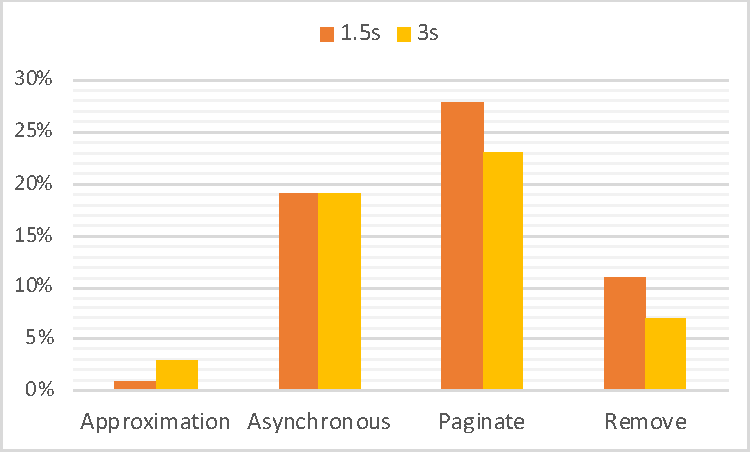
\includegraphics[width=0.8\columnwidth]{figs/preference.pdf}
    \caption{How much better do users like New pages?}
    \label{fig:userstudy_diff}
\end{figure}
\begin{figure}[h]
    \centering
    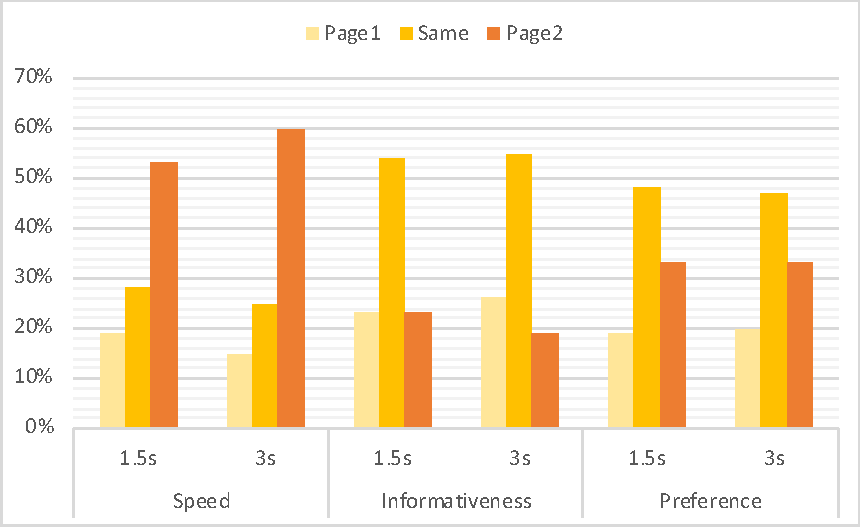
\includegraphics[width=0.8\columnwidth]{figs/user-study.pdf}
    \caption{How people prefer the pages?}
    \label{fig:userstudy}
\end{figure}
\fi

\subsubsection{User study results}
A summary of the user study results is shown in Table \ref{tab:userstudy_diff}, and the questionnaire and raw data are available on Panorama webpage \cite{userstudydata}.
%, there are always some participants who think Base is better, and some think New is better, and some think two versions are similar. \alvin{just say the results are mixed?}
In this table, we show the percentage of users who
think New is better minus those who think Base is better,
which we refer to as the {\it net} benefit of the new design, for every type of refactoring and every
question (Performance, Functionality, and Overall).
Users are given the two pages in random order, and are not aware of the view-design difference between the two pages in advance.

A short answer to our research question is ``Yes''. In fact, for all type
of view-changing optimization, users think the New design is {\it not worse}
than the Base design. Particularly, for {\it asynchronous} loading,
{\it pagination}, and {\it removal}, the new designs clearly win more users
than the baseline designs.

In terms of performance, the net win for the New design is clear. Many users
indeed notice the 1.5-second difference in the page-load time. In 10 out of 12 cases, \alvin{show \%?}
the New design has a net positive benefit on more than 30\% of the participants.

In terms of functionality, the results are quite interesting. For 
{\it approximation} and {\it pagination}, many users did notice the
content difference, leading to the Base design winning about 10\% of users.
However, for {\it asynchronous} loading and content {\it removal}, surprisingly,
many users neither notice the content difference nor think New design delivers worse contents. It could be that removing contents made the page cleaner to some users. For example, after removing the sidebar in Tracks \alvin{in Tracks? (if tracks is the app name)} (Tr5 in Table \ref{tab:dbsize} \alvin{I can't find case 11 in that table?}), some participants like it because ``Adding the sidebar makes scrolling harder.'' 

In terms of overall perception, the New design has a {\bf net win}.
Among the four types of optimizations, paginations and asynchronous loading
are the most appealing to users, while approximation is the least appealing.

We also conducted another set of user study with another 100 participants,
where we use an even larger (2-10$\times$) database size \alvin{how large?} \junwen{The size get differntly larger for different cases, some are 10 times, some are 2 times, some are 2.5 times} and hence make the page-load time
differences between New design and Base design even bigger (3 seconds).
We do observe that more participants noticed the performance advantage
of the New design. However, we also observe that the overall perception
only goes up a little bit more for the New design. We skip the details for
the space constraints.



\begin{table}[]

\centering
\caption{Net user perception enhancement by New design\\ (\% users 
who prefer New   $-$ \% users who prefer Base )}
\label{tab:userstudy_diff}
\begin{tabular}{@{}lrrrr@{}}
\toprule
                                & Approximation & Asynch & Paginate & Removal  \\ \midrule
Performance       & 23.50\%       & 31.00\%      & 45.00\%  & 35.50\% \\ 
%                             & 3s   & 35.50\%       & 42.00\%      & 45.50\%  & 58.00\% \\ \midrule
Functionality  & -7.50\%       & 17.50\%      & -13.00\% & 5.50\%  \\ 
 %                            & 3s   & -10.50\%       & 10.50\%      & -24.50\%  & -3.00\% \\ \midrule
Overall   & 1.00\%        & 18.50\%      & 28.00\%  & 10.50\% \\  
 %                            & 3s   & 2.50\%        & 19.00\%      & 23.00\%  & 7.00\%  \\ 
 \bottomrule
\end{tabular}
 \vspace{-0.2in}
\end{table}


\iffalse
\begin{table}[]
\centering				
\caption{User Study Result: Why prefers a web page?}
\label{tab:codebook}	\begin{tabular}{@{}clrm{3.5cm}@{}}
\toprule
                                            & Reason        & Num & Example                                           \\ \midrule
\multirow{3}{*}[-10pt]{Page 1}                     & Informative  & 125 & p1 has more  information.             \\ \cmidrule(l){2-4} 
                                            & Faster        & 37  & p1 loads fast.                                \\ \cmidrule(l){2-4} 
                                            & Display Style & 59  &  not paginating  is helpful. \\ \midrule
\multicolumn{1}{l}{\multirow{3}{*}[-10pt]{Page 2}} & Informative   & 83  & p2 has  more information.             \\ \cmidrule(l){2-4} 
\multicolumn{1}{l}{}                        & Faster        & 215 & p2 loads much faster.                         \\ \cmidrule(l){2-4} 
\multicolumn{1}{l}{}                        & Display Style & 168 & I like paginating.         \\ \bottomrule
\end{tabular}
\end{table}
\fi
\iffalse
\emph{Discussion.} The baseline page load time greatly affects people's attitude towards end-to-end time consumption. It's because of the non-uniform Internet status and human sense of time. In addition, longer loading time is, the more information on web-page the participant is expecting. During the experiment, we also found that participants have a strong preference towards pagination. Some of them think pagination is a clean UI design, while the others regard it as an obstacle to searching.
%[does the base line page-load time affect people's reaction?] [Does the users' reaction differ for different types of view-changes?]

\fi


\vspace{-0.05in}
\subsection{RQ4: how accurate is the \Tool estimator?}
We use the web page shown in Figure \ref{fig:heatmap} as a case study.
15 HTML tags on this page render dynamically generated contents.
With 200 database records, dynamic profiling shows that
the story tag is the top performance bottleneck, followed by the guideline
tag and then the message-count the cheapest. When the workload increases to
2000 and 20000 records, dynamic profiling shows that the guideline
tag is the top bottleneck, followed by the story tag. These results match
the performance gains we can get by optimizing these three tags: 
using 20000 records, asynchronously
loading or removing the guideline text can reduce the page end-to-end 
load time by more than 1 second; 
paginating the story-tag can speed up the page load time
by about 100 milliseconds; approximating the message count does not change page load time.

The static mode of \Tool estimator can indeed predict performance bottleneck
without running the application --- the guideline text gets the
highest complexity score (5) among all 15 tags, followed by the story tag (4), and then the
message-count tag (3), with the remaining 12 tags
getting 0 points.


\iffalse
\begin{table}[]
\centering
\caption{Performance cost ranking (static vs dynamic)}
\label{tab:cons1}
\begin{tabular}{@{}lrrrrrrr@{}}
\toprule
 & \multicolumn{2}{l}{200} & \multicolumn{2}{l}{2000} & \multicolumn{2}{l}{20000} & \multicolumn{1}{l}{static} \\ \midrule
guideline & \cellcolor[HTML]{C0C0C0}2 & 2 & \cellcolor[HTML]{C0C0C0}1 & 1 & \cellcolor[HTML]{C0C0C0}1 & 1 & 1 \\ \midrule
tags & \cellcolor[HTML]{C0C0C0}1 & 1 & \cellcolor[HTML]{C0C0C0}2 & 2 & \cellcolor[HTML]{C0C0C0}2 & 2 & 2 \\ \midrule
msg\_count & \cellcolor[HTML]{C0C0C0}3 & 3 & \cellcolor[HTML]{C0C0C0}3 & 3 & \cellcolor[HTML]{C0C0C0}3 & 3 & 3 \\ \bottomrule
\end{tabular}
\end{table}
\fi


%%%%%%COMMENT OUT%%%%
\begin{comment}

\begin{table}[]
\centering
{\small					
\caption{User Study Result: How people prefer the pages?}
\label{tab:userstudy}	
\begin{tabular}{@{}llrrrr@{}}
\toprule
 &  & \multicolumn{1}{l}{page1} & \multicolumn{1}{l}{same} & \multicolumn{1}{l}{page2} & \multicolumn{1}{l}{diff} \\ \midrule
Speed & 1.5s & 19.00\% & 28.25\% & 52.75\% & 33.75\% \\ \midrule
 & 3s & 15.13\% & 24.50\% & 60.38\% & 45.25\% \\ \midrule
Info&1.5s & 22.63\% & 54.13\% & 23.25\% & 0.63\% \\ \midrule
 & 3s & 26.00\% & 54.88\% & 19.13\% & -6.88\% \\ \midrule
Prefer & 1.5s & 18.88\% & 47.75\% & 33.38\% & 14.50\% \\ \midrule
 & 3s & 20.00\% & 47.13\% & 32.88\% & 12.88\% \\ \bottomrule
\end{tabular}
}
\end{table}

\end{comment}

\subsection{Threats to validity}
Threats to the validity of our work could come from multiple
sources. 
\textbf{Internal Validity}: The HTML tags that are dynamically generated through JavaScript can not be detected or analyzed by \Tool. \textbf{External Validity}: The 12 applications in our benchmark suite may not represent all real-world applications; The synthesized databases may not represent real-world workloads; The machine and network settings of our profiling may differ from real users’ setting; the 100 participants of our user-study from MTurk may not represent all real-world users. Overall, we have tried our best to conduct an unbiased study.




\section{Threats to validity}

\textbf{Threats to validity.}
As discussed in Section \ref{sec:approach}, 
\Tool may raise false alarms in rare cases.
%although we have not observed these cases in practice.
%Both Rails and Django allow developers to use special key words to declare non-persistent fields in a model class. In rare cases, a table column may be deleted from table, while a non-persistent field with the same name could be added to the same class. 
%Besides schema, it's possible for developers to define the classes' fields in multiple manners. For example Django allows using @property decorator on a function so that a class can use it as a field and Rails has similar API attr\_accessor. The application code that refers to those fields might be considered as inconsistent code incorrectly. We already tried our best to eliminate their influence in our tool design. But due to the flexibility of the languages, there might left some cases that our tool cannot handle.
%In addition to what already discussed in Section \ref{sec:approach}, 
There are also sources of false negatives.
%Firstly, the query extraction relies on type inference which only works within a file, it's possible to miss queries that are issued across files. Secondly, 
%the code parsing relies on existing parser libraries (pyparser for Django, and yard for rails), 
Application code that cannot be parsed by pyast or Yard cannot be analyzed by 
\Tool. A schema may be changed by SQL commands issued directly to the database
without any record in migration files. This is considered a bad  practice~\cite{migration-guide} and is not handled by \Tool.
A schema may also be changed in migration files 
through raw SQL commands wrapped in ORM APIs like
\texttt{migrations.RunSQL(...)} in
Django and \texttt{migrations.execute(...)} in Rails. 
This feature is rarely used by web developers (less than 1\% of cases in our study), and is not handled by \Tool.
If the new version adds a table \texttt{T}, and then changes the schema about 
\texttt{T} or its columns, indices, or
associations, \Tool would not check whether the new code is consistent with the
schema of \texttt{T}, as \texttt{T} does not exist in the old version.
Finally, what we observed in the 12 Rails and Django applications may not apply to
other open-source applications.

% \junwen{Why cannot we keep a record of functions with @property decorator, and remove the false positive}

% \junwen{Add the developers change code after schema change}
% \textbf{Django limitations.} Functions with the @property decorator that queries can refer to can create false positives for \Tool{}. For example, if a column is deleted but a function with an @property decorator that has the same name as that deleted column is created, \Tool{} will mark queries that refer to the function as queries that incorrectly refer to the schema. Thus, \Tool{} incorrectly raises these queries as errors because of the @property decorator (should I include an example). More generally, tables/columns/association relationships/indexes that are not recorded in an application’s migrations will not be included in the \Tool{}’s schema extraction and therefore there might be some false positives that arise. Annotations applied to a schema by a query in which the name of said annotation is the same as a deleted/renamed column can create false positives because that new annotation is not recorded in the extraction of the app’s schema. \Tool{} also requires python version >= 3.9.4 to be able to run.

\section{Related Work}

%%
%% The next two lines define the bibliography style to be used, and
%% the bibliography file.
\bibliographystyle{ACM-Reference-Format}
\bibliography{ref}

%%
%% If your work has an appendix, this is the place to put it.
\end{document}
\endinput
%%
%% End of file `sample-authordraft.tex'.
